\section{A New Framework for On-Stack Replacement}

Modern language runtimes dynamically adapt the execution to the actual workload, maintaining different versions of the code generated with different, often speculative, optimizations. For this reason, they typically implement on-stack replacement mechanisms to dynamically transfer execution between them {\em while} a version of the method to optimize is still running.

Pioneered in the SELF language runtime in the early 90's, OSR mechanisms have drawn considerable attention from the community of VM builders as the Java language grew popular. OSR is nowadays used in a relevant number of virtual machines to implement optimization techniques such as profile-driven and deferred compilation, and can also be employed to support debugging of optimized code.

\noindent OSR can be a very powerful tool for implementing dynamic languages, for which most effective optimization decisions can typically be made only at run time, when critical information such as type and shape of objects becomes available. In this scenario, OSR becomes useful also to perform deoptimization, i.e. when the running code has been speculatively optimized and the assumption used for the optimization does not hold anymore, the optimized function is interrupted and the execution continues in a safe version of the code.

In this thesis, we propose a general-purpose, target-independent framework for OSR. Specific goals of our solution include:
\begin{itemize}[parsep=0pt]
\item The ability for a function reached via OSR to fire an OSR itself: this would allow switching from a base function $f$ to an optimized function $f'$, and later on to a further optimized version $f''$, and so on.
\item Supporting deoptimization, i.e., transitions from an optimized function to a less optimized function from which it was derived.
\item Supporting transitions at arbitrary program points, including those that would require adjusting the transferred program state to resume the execution in the OSR target function.
\item Supporting OSR targets either generated at run-time (e.g., using profiling information) or already known at compilation time.
\item Hiding from the front-end that generates the different function versions all the implementation details for handling OSR transitions between them.% at specific points.
\end{itemize}

\noindent We show the feasibility of our approach by implementing \osrkit, a prototype library for the MCJIT just-in-time compiler from the LLVM compiler infrastructure.

\subsection{Approach}

The key to generality and platform-independence in our approach is to express the OSR machinery entirely at intermediate representation (IR) level, without resorting to native-code manipulation or special intrinsics of a compiler.

\ifdefined\noauthorea
\begin{figure}[hb]
\begin{center}
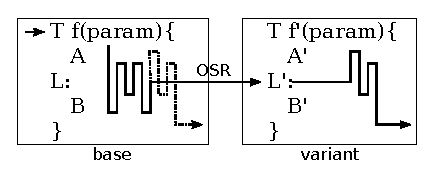
\includegraphics[width=0.7\textwidth]{figures/osr-dynamics/osr-dynamics.eps}
\caption{\protect\label{fig:osr-dynamics} On-stack replacement dynamics: control is transferred via OSR from a point \textsf{L} of a base function \textsf{f} to a point \textsf{L'} in a variant \textsf{f'} of \textsf{f}.}
\end{center}
\end{figure}
\fi

\noindent Consider the generic OSR scenario shown in \myfigure\ref{fig:osr-dynamics}. A base function \fbase\ is executed and it can either terminate normally (dashed lines), or an OSR event may transfer control to a variant \fvariant, which resumes the execution. The decision of whether an OSR should be fired at a given point \osrpoint\ of \fbase\ is based on an {\em OSR condition}. A typical example in JIT-based virtual machines is a profile counter reaching a certain hotness threshold, which indicates that \fbase\ is taking longer than expected and is worth optimizing. Another example is a guard testing whether \fbase\ has become unsafe and execution needs to fall back to a safe version \fvariant. This scenario includes deoptimization of functions generated with aggressive speculative optimizations. 

%In this section we present 
%On-stack replacement is used in mainstream runtime systems to support a number of powerful techniques such as profile-driven optimization, 